\section{Motorstyring }\label{sec:sec_motorstyring}
Målinger af vognens dynamik, der blev gennemgået i afsnit \ref{sec:sec_motoroverforelse}, er baseret på stepresponset af vognen ved en konstant spænding, men med faste strømbegrænsninger i intervaller.
Dette giver anledning til at vægle en motorstyring der sørger for en konstant strøm til motoren.
Således vil udgangssignalet fra regulatoren i form af en reguleringsspænding, $V_{reg}$ omsættes i motorstyringen til den ønskede strøm $I_{reg}$, der igen giver den ønskede acceleration $a_v$ af vognen.  

\subsection{Design af motorregulering}
\begin{wrapfigure}{r}{0.5\textwidth}
	\centering
	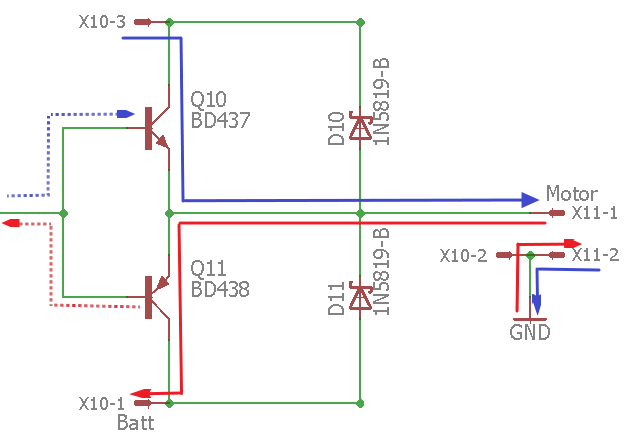
\includegraphics[width=.45\textwidth]{billeder/motor_bidirectional.png}
	\caption{Strømretninger ved positiv (blå) og negativ (rød) styresignal igennem BJT transistorne.}
	\label{fig:motor_bidirectional}
\end{wrapfigure}
Da DC-motoren er en kompleks enhed, hvis dynamik og opbygning ligger uden for opfanget af denne rapport. 
I figur \ref{fig:motor_diagram} ses det samlede kredsløb af motorreguleringen.
I motorstyringen anvendes en simpel feedback regulering af strømmen igennem en NPN \emph{(Q10)} og PNP \emph{(Q11)} transistor, således at forholdet mellem indgangssignalet og udgangsstrømmen til motoren holdes konstant.
Motorstyringen er opbygget som en såkaldt \textit{ Bi-directional DC motor driver} som gør det muligt at styre retningen af strømmen igennem motoren.
Således vil et positivt styresignal åbne for strømmen fra $+8V Batt$ igennem NPN transistoren \emph{(Q10)} ud til motoren, og et negativt styresignal vil åbne for strømmen fra $GND$ igennem PNP transistoren \emph{(Q11)} til $-8V Batt$, se figur \ref{fig:motor_bidirectional}.

\begin{figure}[h!]
	\centering
	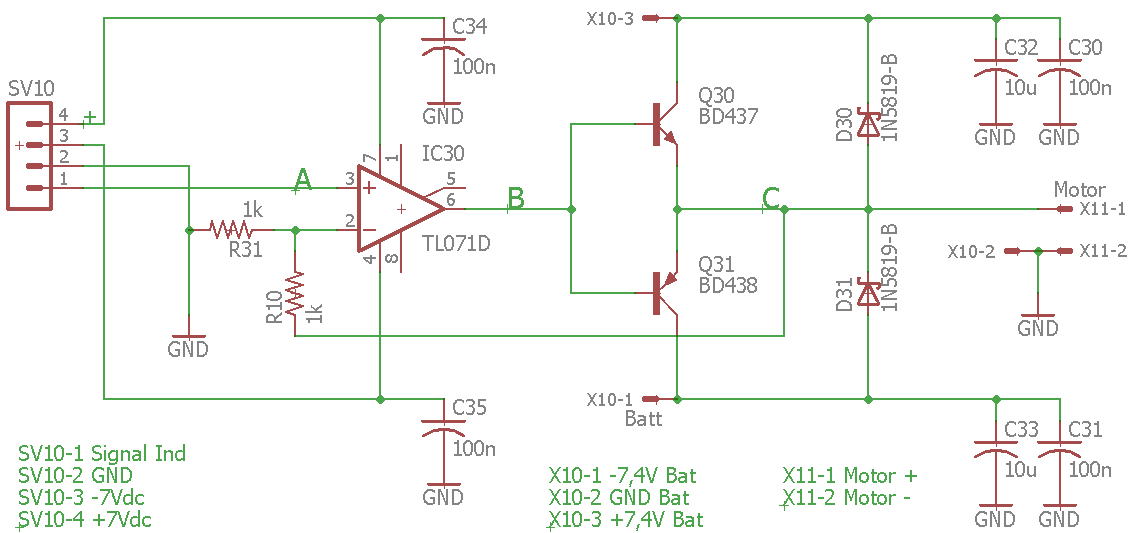
\includegraphics[width=1\textwidth]{billeder/motor_cont_schematic.png}
	\caption{Diagram af motor styringen}
	\label{fig:motor_diagram}
\end{figure}
\FloatBlock

For at håndtere de transiente spændings udslag der måtte komme fra motor, idet den som spole er en induktiv belastning på udgangen, er der i kredsløbet anbragt to såkalde \textit{flyback} eller friløbs dioder \emph{(D10)} og \emph{(D11)}.
Det er valgt at bruge en \textit{Schottky} \emph{1N5819} diode, da denne har et lavere spændingsfald og en hurtigere \textit{reverse recovery}.


\subsection{Beregninger og dimensionering}


\husk{JJ}{beregninger af forhold mellem spænding og strøm i regulatoren}
\husk{JJ}{PSpice simulering af regulator}

\subsection{Overførelsesfunktion af motor}
For at bestemme dynamikken af DC-motoren opstilles en forenklet model af motoren.

\begin{figure}[h!]
	\centering
	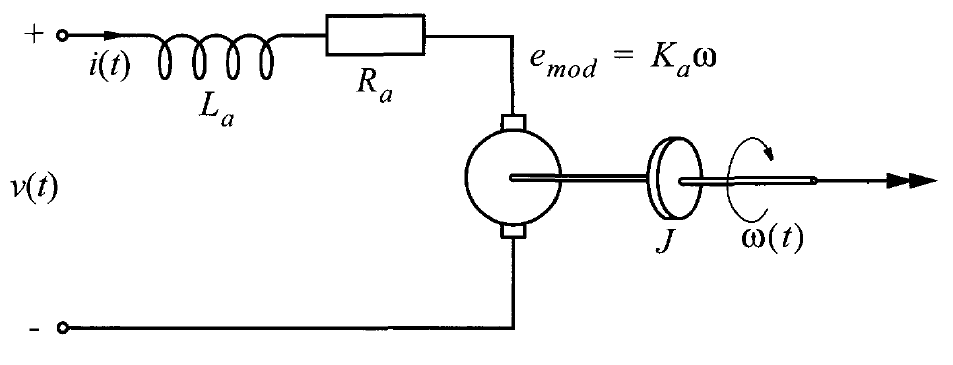
\includegraphics[width=.6\textwidth]{billeder/motor_model.png}
	\caption[Model af elektromotorisk system til brug ved modellering af motor]{Model af elektromotorisk system til brug ved modellering af motor\protect\footnotemark.}
	\label{fig:motor_model}
\end{figure}
\FloatBlock
\footnotetext{Figuren er tilrettet fra \cite[Figur 2.16, s. 52]{Reg2015}}

Ved at fastholde motoren, således at den mod-elektromotoriskekraft ($e_{mod}$) kan sættes til nul dvs. $\omega = 0$, er det muligt at måle motores induktans.
Modellen kan således omstilles som
\begin{align}
	v(t) = R_ai(t) + L_a\dfrac{di(t)}{dt}
\end{align}
Måling af strømmen igennem motoren er forstaget over en $0,2 \si{\ohm}$ test-modstand
\footnote{Modstand med meget lille induktans}.
Motorens egen modstand er målt til $R_{motor} = 3,2 \si{\ohm}$, hvilket giver en samlet modstand på $R_a = R_{test} + R_{motor} = 3,4 \si{\ohm}$ i test opstillingen. 
\begin{figure}[h!]
	\centering
	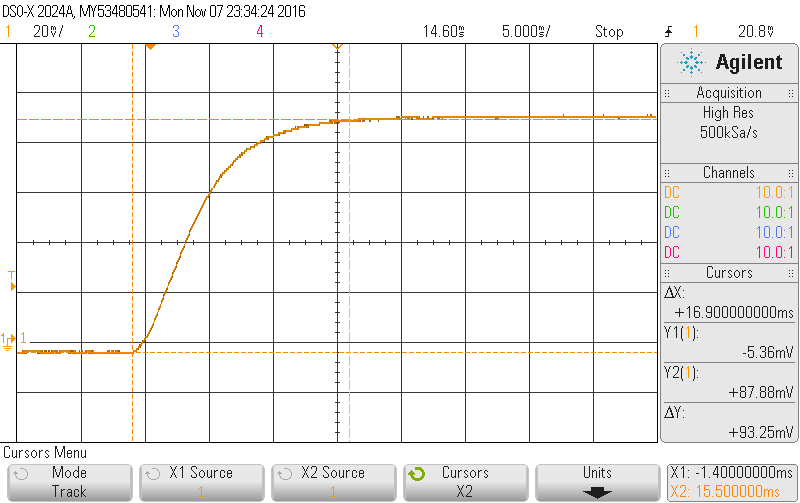
\includegraphics[width=.8\textwidth]{billeder/motor_L.png}
	\caption{Måling af transient forløb for strømmen igennem DC-motor.}
	\label{fig:motor_dynamik_scoop}
\end{figure}
Tidskonstanten for ladning af en spole er, $\tau = \frac{L}{R}$.
For at bestemme $L$, måles tiden $t$ ved $5\tau$ som er ved
\begin{align}
	\% opladning = \left( 1 - \frac{1}{e^{t/\tau}} \right) \cdot 100\% \Rightarrow  \left( 1 - \frac{1}{e^{t/5}} \right) \cdot 100 \approx 99,32\% 
\end{align}
derefter kan $L_a$ bestemmes som, ved aflæst tid på $16,9\si{\milli\second}$ i fig. \ref{fig:motor_dynamik_scoop} 
\begin{align}
	5\tau = \frac{L_a}{R_a} \Rightarrow L_a = 16,9\si{\milli\second} \cdot 3,4 \si{\ohm} = 57,5 \si{\milli\henry}
\end{align}
Overførelsesfunktion for motoren opstilles som
\begin{align}
H_{motor} = \frac{V_o}{V_i} = \frac{s L_a}{s L_a + R_{motor}} = \frac{ \frac{L_a}{R_{motor}}s}{ \frac{L_a}{R_{motor}}s +1} = \frac{\num{18E-3}s}{\num{18E-3}s +1} \label{eq:motor_trans}
\end{align}  



